\label{sec:case}
\lstdefinestyle{casecodestyle}{
  language=C,
  basicstyle=\ttfamily\fontsize{7pt}{7.4pt}\selectfont,
  keywordstyle=\color{figgraytext}\bfseries,
  keywordstyle=[2]\color{figcontract!80!black}\bfseries,
  keywordstyle=[3]\color{figloop!75!black}\bfseries,
  commentstyle=\color{figcontract!78!black},
  stringstyle=\color{figgraytext},
  identifierstyle=\color{black},
  morekeywords=[2]{requires,ensures,assigns,logic,integer,assert,valid,separated,result,old,at,Pre,true,nothing,decreases},
  morekeywords=[3]{loop,invariant},
  emph={AutoSpec,SESpec,unknown,product,Fib,gcd,gcd_logic,malloc,free},
  emphstyle=\color{figcall!75!black},
  backgroundcolor=\color{overviewgray},
  frame=single,
  frameround=tttt,
  rulecolor=\color{figgrayframe},
  framerule=1pt,
  xleftmargin=1mm,
  xrightmargin=1mm,
  framexleftmargin=1mm,
  framexrightmargin=1mm,
  breaklines=true,
  breakatwhitespace=false,
  columns=fullflexible,
  keepspaces=true,
  showstringspaces=false,
  aboveskip=0pt,
  belowskip=0pt
}
\lstdefinestyle{casecompactstyle}{
  style=casecodestyle,
  basicstyle=\ttfamily\fontsize{5pt}{5.3pt}\selectfont,
  xleftmargin=0.5mm,
  xrightmargin=0.5mm,
  framexleftmargin=0.5mm,
  framexrightmargin=0.5mm
}
\lstdefinestyle{caseinnerstyle}{
  style=casecodestyle,
  frame=none,
  backgroundcolor=\color{overviewgray},
  rulecolor=\color{overviewgray},
  xleftmargin=0pt,
  xrightmargin=0pt,
  framexleftmargin=0pt,
  framexrightmargin=0pt
}
\lstdefinestyle{casecompactinnerstyle}{
  style=casecompactstyle,
  frame=none,
  backgroundcolor=\color{overviewgray},
  rulecolor=\color{overviewgray},
  xleftmargin=0pt,
  xrightmargin=0pt,
  framexleftmargin=0pt,
  framexrightmargin=0pt
}

The case studies below show, on concrete programs, what symbolic execution contributes to generated specifications. To keep the main text focused, we present five representative cases here and defer five supplementary cases to the supplementary material. Across all cases, \toolname\ reuses the same local symbolic context and template-routing signals, so each main case emphasizes a distinct role of that context rather than repeating the full mechanism.

Table~\ref{tab:case-study-map} summarizes the organization. The main cases cover phase-split loop invariants, path-complete postconditions under C aliasing, recursive heap shape specifications, the contrast between RTE-safety and functional specification, and the scale boundary on industrial control code. The supplementary material retains the factorial, GCD, MulLoop, Ackermann, and matrix-multiplication details as supplementary evidence.

\begin{table}[H]
  \centering
  \caption{Organization of the case studies.}
  \label{tab:case-study-map}
  \begin{adjustbox}{max width=\linewidth}
  \begin{tabular}{lll}
    \toprule
    \textbf{Case} & \textbf{Location} & \textbf{Main lesson} \\
    \midrule
    SyGuS loop & Main text & Phase-split invariant from weak goals \\
    TripleAbsMax & Main text & Path-complete C/ACSL postconditions \\
    Linked list & Main text & Shape-predicate routing \\
    Linear search & Main text & RTE-safety vs.\ functional specification \\
    Industrial pipeline & Main text & Scale and verifier boundary \\
    Factorial, GCD & Supplementary & Inductive helper summaries \\
    MulLoop & Supplementary & Prior-tool contextual example \\
    Ackermann & Supplementary & ACSL/SMT recursion boundary \\
    Matrix multiply & Supplementary & Nested loops; verifier/SMT-timeout boundary \\
    \bottomrule
  \end{tabular}%
  \end{adjustbox}
\end{table}

In the figures below, ACSL annotations enclosed by $/*@\cdots */$ are generated by \toolname\ and then retained after verification or pruning.


%Note that in all figures, the black boxes highlight the portions generated by the LLM, while the remaining elements are automatically derived through symbolic execution.

\subsection{Case 1: Phase-Split Invariant from a Weak Goal}

\begin{figure}[!t]
    \centering
    \begin{tcolorbox}[casebox, title={Case 1: symbolic state exposes loop phases}]
\begin{lstlisting}[style=caseinnerstyle]
int unknown();

/*@ requires n > 0; */
void SyGuS38(int n) {
  int c = 0;

  /*@
    loop invariant ((c == 0)&&(n == \at(n,Pre))) || (1 <= c <= n) ;
    loop invariant n == \at(n,Pre);
    loop assigns c ;
  */
  while (unknown()) {
    if(c == n) {
      c = 1;
    }
    else {
      c = c + 1;
    }
  }

  /*@ assert (c == n) ==> (c >= 0); */
}
\end{lstlisting}
    \end{tcolorbox}
    \caption{Case 1 (SyGuS-38): a nondeterministic loop whose phase structure is exposed by symbolic execution.}
    \label{fig:case1}
\end{figure}

Fig.~\ref{fig:case1} isolates the benefit of symbolic execution when the assertion is too weak to guide invariant synthesis. The goal $(c = n) \Rightarrow (c \ge 0)$ can be proved by many uninformative invariants; what matters here is the loop's phase structure.

At the loop boundary, symbolic execution separates the unentered state (\texttt{c == 0}) from the inductive region (\texttt{1 <= c <= n}) and records that \texttt{n} is stable. The disjunctive template instantiates exactly that split, yielding an invariant that describes the loop behavior rather than merely satisfying the final assertion.

\subsection{Case 2: Path-Complete Postconditions \rev{for Pointer-Manipulating Code}}

\begin{figure}[!t]
    \centering
    \begin{tcolorbox}[casebox, title={\textcolor{white}{Case 2: path-complete postconditions for pointer-manipulating code}}, width=\linewidth]
\begin{lstlisting}[style=casecompactinnerstyle]
typedef struct __TripleAbsMax
{
  int abs[3];
  int tmax;
  int* ret;
} TripleAbsMax;

/*@
  requires \valid(pIp);
  requires \valid(pIp->abs+(0..2)) ;
  requires \valid(pIp->ret);
  requires \separated(pIp, pIp->ret);

  ensures pIp->ret == \old(pIp->ret);
  ensures -pIp->abs[2] <= pIp->abs[1] && pIp->abs[0] <= pIp->abs[1] && pIp->abs[2] < 0 && pIp->abs[1] >= 0
  && pIp->abs[0] >= 0 ==> pIp->tmax == pIp->abs[1] && *\old(pIp->ret) == pIp->abs[1];
  ... all 32 paths

  assigns pIp->tmax, *(pIp->ret);
*/
void TripleAbsMaxFun(TripleAbsMax *pIp)
{
  int absfx1 = pIp->abs[0];
  int absfy2 = pIp->abs[1];
  int absfz3 = pIp->abs[2];

  if (pIp->abs[0] < 0){  absfx1 = -pIp->abs[0];}

  if (pIp->abs[1] < 0){  absfy2 = -pIp->abs[1];}

  if (pIp->abs[2] < 0){  absfz3 = -pIp->abs[2];}

  if (absfx1 > absfy2){  pIp->tmax = absfx1;}
  else{ pIp->tmax = absfy2; }

  if (absfz3 > pIp->tmax){pIp->tmax = absfz3;}

  *(pIp->ret) = pIp->tmax;
}

/*@
  requires \valid(pIp);
  requires \valid(pIp->abs+(0..2));
  requires \valid(pIp->ret);
  requires \separated(pIp, pIp->ret);
*/
void main1(TripleAbsMax *pIp)
{
  pIp -> abs[0] = 1;
  pIp -> abs[1] = 2;
  pIp -> abs[2] = -3;

  TripleAbsMaxFun(pIp);

  /*@ assert pIp -> tmax == 3; */
}
\end{lstlisting}
    \end{tcolorbox}
    \caption{Case 2 (TripleAbsMax): \rev{a loop-free program with 32 feasible paths under the precondition shown.}}
    \label{fig:case3}
\end{figure}

Fig.~\ref{fig:case3}, from our \textbf{pIp} benchmark, is the main C-specific case. The function computes the maximum absolute value of three struct-stored integers and writes it both to \texttt{pIp->tmax} and through \texttt{pIp->ret}.

\rev{Starting from the default precondition, including \texttt{\textbackslash separated(pIp, pIp->ret)}, symbolic execution derives the guarded postconditions for the feasible paths.}
\subsection{Case 3: Shape-Predicate Routing for Linked Structures}

\begin{figure}[!t]
    \centering
    \begin{tcolorbox}[casebox, title={Case 3: route-selected shape predicates}]
\begin{lstlisting}[style=caseinnerstyle]
struct SLL {
    struct SLL *tail;
    int head;
};

/*@
  predicate lseg{L}(struct SLL* x, struct SLL* y) =
    x == y || (x != y && \valid(x) && \separated(x, y) && lseg{L}(x->tail, y));
*/

/*@ predicate listrep(struct SLL* head) = lseg(head, \null); */

/*@
  logic integer list_length{L}(struct SLL* x) =
    (x == \null) ? 0 : 1 + list_length{L}(x->tail);
*/

/*@
  requires listrep(l);
  requires \valid_read(&data);
  assigns \nothing;
  ensures listrep(l);
  ensures \result == l;
*/
struct SLL * main1(struct SLL *l, int data)
{
    struct SLL *p;
    p = l;

    /*@
      loop invariant listrep(p);
      loop invariant listrep(l);
      loop invariant lseg(l, p);
      loop invariant data == \at(data,Pre);
      loop invariant l == \at(l,Pre);
      loop invariant list_length(l) >= list_length(p);
      loop assigns p;
    */
    while (p) {
      if (p->head == data) {
        /*@ assert data == \at(data,Pre); */
        /*@ assert l == \at(l,Pre); */
        return l;
      }
      p = p->tail;
    }

    return l;
}
\end{lstlisting}
    \end{tcolorbox}
    \caption{Case 3 (linked-list traversal): a recursive data-structure program with shape predicates.}
    \label{fig:case4}
\end{figure}

Fig.~\ref{fig:case4} illustrates template routing rather than another scalar invariant pattern. The loop walks a singly linked list and returns the original head pointer, so ACSL needs an explicit heap-shape abstraction instead of only arithmetic facts.

Symbolic execution identifies \texttt{p} as the advancing list pointer and records the local update facts, while the static route recognizes the recursive type and field-access pattern. That route selects the recursive-shape template, which supplies \texttt{lseg}, \texttt{listrep}, and \texttt{list\_length}; the loop template then connects the original head to the current suffix through \texttt{lseg(l, p)}. The key point is that the shape predicates are injected through a program-structure route and then anchored by symbolic cursor facts, rather than invented from source text alone.

\subsection{Case 4: RTE Safety vs. Functional Specification}
\label{app:case-search}

We reuse the linear search example from Fig.~3 of Preguss~\cite{Wang2025ATO} and run \toolname\ on the same source. The point is not a head-to-head accuracy comparison: Preguss is driven by RTE-safety obligations, while \toolname\ attempts to generate goal-independent functional specifications. This distinction also affects failure handling. On the Frama-C validation side, \toolname\ records potential RTE reports as warnings rather than treating RTE elimination as the main target. On the QCP side, however, an RTE can still block symbolic execution; the flattened-memory default precondition covers validity, bounds, and separation facts exposed by the model, but it does not guarantee that every arithmetic or pointer-related RTE is avoided. The refinement stage can ask the LLM to strengthen preconditions to avoid such failures, but this is a supporting mechanism for functional specification generation rather than the objective itself.

\begin{figure}[!t]
  \centering
  \begin{tcolorbox}[casebox, title={Preguss: RTE-guided safety specification}, width=0.96\linewidth]
\begin{lstlisting}[style=casecompactinnerstyle]
/*@ requires \valid_read(arr+(0..len-1));
    assigns \nothing; */
int * search(int * arr, int len, int val) {
    int i = 0;
    /*@ loop assigns i; */
    while (i < len) { ... }
}
\end{lstlisting}
  \end{tcolorbox}
  \vspace{1.4ex}

  \begin{tcolorbox}[casebox, title={\toolname: verifier-checked prefix-search specification}, width=0.96\linewidth]
\begin{lstlisting}[style=casecompactinnerstyle]
/*@ logic integer count_eq{L}(int* a, integer lo,
      integer hi, integer v) =
      lo >= hi ? 0 : count_eq(a, lo, hi - 1, v)
                   + (a[hi - 1] == v ? 1 : 0); */
/*@ requires \valid(arr + (0 .. len - 1));
    requires len >= 0;
    ensures \forall integer k; 0 <= k < len ==>
              arr[k] == \at(arr[k], Pre);
    ensures \result == \null ==>
              count_eq(arr, 0, len, val) == 0;
    ensures \result != \null ==>
              count_eq(arr, 0, \result - arr, val) == 0
              && *\result == val;
    assigns \nothing; */
int * search(int * arr, int len, int val) {
    int i = 0;
    /*@ loop invariant 0 <= i <= len;
        loop invariant \forall integer k;
            0 <= k < len ==> arr[k] == \at(arr[k], Pre);
        loop invariant count_eq(arr, 0, i, val) == 0;
        loop assigns i; loop variant len - i; */
    while (i < len) {
        if (arr[i] == val) return arr + i;
        i = i + 1;
    }
    return (int *)0;
}
\end{lstlisting}
  \end{tcolorbox}
  \caption{Case 4 (linear search). Preguss verifies memory-access safety; \toolname\ also captures the prefix-search property and returned-pointer consequence.}
  \label{fig:case7}
\end{figure}

Fig.~\ref{fig:case7} shows the difference in target. Preguss emits the memory-safety precondition needed to discharge \texttt{arr[i]} accesses. \toolname\ instead routes the loop to a count-occurrences helper and records both return cases: null means \texttt{val} is absent, and non-null means the returned pointer dereferences to \texttt{val} with no earlier occurrence. This illustrates why RTE-safety synthesis of Preguss~\cite{Wang2025ATO} and our functional specification synthesis should not be read as identical tasks.

\subsection{Case 5: Industrial Pipeline Stress Test}
\label{subsec:case9-ip}

\begin{figure*}[!t]
    \centering
    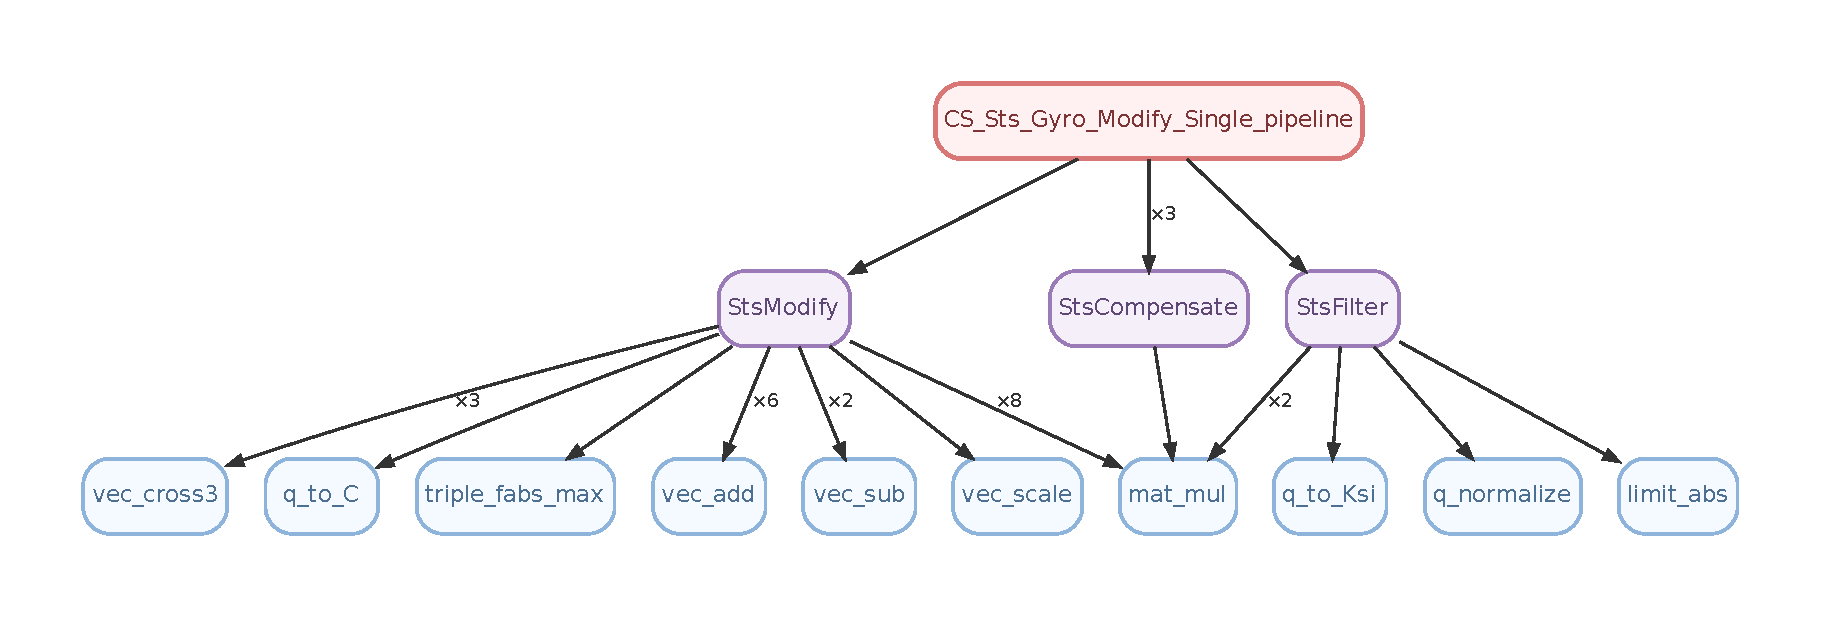
\includegraphics[width=0.95\textwidth]{images/ip_callgraph.pdf}
    \caption{Call graph of the single-star-sensor filter-update pipeline. Edge labels show call multiplicity; unlabeled edges are $\times 1$.}
    \label{fig:case9-callgraph}
\end{figure*}

\smallskip
\noindent\textbf{Program structure.}
We applied \toolname\ to a 225-line C transcription of an industrial single-star-sensor Kalman-update pipeline. The translation unit contains 14 functions, 33 call sites, and 8 loops; the entry delegates to three pipeline stages, which in turn call ten numeric and quaternion helpers (Fig.~\ref{fig:case9-callgraph}). This case is included to show the scale boundary, not another single function invariant pattern.

\smallskip
\noindent\textbf{What \toolname\ produced.}
Driven by \texttt{gpt-5.4-mini} at maximum reasoning effort (\texttt{reasoning\_effort=high}) in the goal-independent configuration, \rev{\toolname\ completed specification generation for 13 of the 14 functions.} The assembled file contains 198 ACSL clauses, and Frama-C/WP discharges 601 of 625 verification conditions ($96.2\%$) at a 30\,s per-goal timeout. Table~\ref{tab:case9-wp} shows that increasing the timeout from 5\,s to 30\,s recovers only one additional goal, so the residual failures reflect hard proof obligations rather than transient budget noise.

\rev{Because proof discharge alone does not measure specification informativeness, we also manually audited the accepted contract of each function. We count a postcondition as functional only when it gives a non-vacuous relation between the output or return value and the inputs; \texttt{ensures \textbackslash true} receives no such credit. Ten functions have functional postconditions: \texttt{limit\_abs}, \texttt{q\_to\_C}, \texttt{q\_to\_Ksi}, \texttt{triple\_fabs\_max}, \texttt{vec\_cross3}, \texttt{vec\_scale}, \texttt{vec\_add}, \texttt{vec\_sub}, \texttt{StsCompensate}, and \texttt{StsFilter}. The other four lack a complete functional summary: \texttt{StsModify} provides only output bounds, \texttt{mat\_mul} has the vacuous \texttt{ensures \textbackslash true}, and the no-op helper \texttt{q\_normalize} and the top-level \texttt{CS\_Sts\_Gyro\_Modify\_Single\_pipeline} have no explicit accepted contract.}

\begin{table}[!t]
  \centering
  \caption{Frama-C/WP proof obligations for the aerospace pipeline.}
  \label{tab:case9-wp}
  \begin{tabular}{lrrr}
    \toprule
    & \multicolumn{3}{c}{\textbf{per-goal timeout}} \\
    \cmidrule(lr){2-4}
    \textbf{Disposition} & \textbf{5\,s} & \textbf{10\,s} & \textbf{30\,s} \\
    \midrule
    Total       & 625           & 625           & 625           \\
    Valid       & 600           & 601           & 601           \\
    Unknown     & 2             & 2             & 3             \\
    Timeout     & 23            & 22            & 21            \\
    \midrule
    Discharge rate & $96.0\%$ & $96.2\%$ & $96.2\%$ \\
    \bottomrule
  \end{tabular}
\end{table}

\smallskip
\noindent\textbf{Boundary exposed.}
\rev{The functions with functional summaries are mostly arithmetic leaves whose semantics admit closed-form ACSL relations, such as \texttt{limit\_abs}, \texttt{vec\_cross3}, and \texttt{q\_to\_C}.} The hard cases are delegate functions and matrix-style loops: composing multi-stage callee summaries and expressing row-major matrix products require either user-provided logic summaries or proof automation beyond the current SMT-only backend. \rev{Thus the $96.2\%$ discharge rate measures verifier acceptance of the generated annotations, while the contract audit separately exposes how much functional behavior those annotations capture.} Concretely, the undischarged goals concentrate in the matrix-multiply leaf \texttt{mat\_mul} and its callers, exactly the triple-nested product dissected in the supplementary material, where the recursive \texttt{mat\_sum} over nonlinear indices makes Z3 time out and the accepted specification degrades to \texttt{ensures \textbackslash true}.
